%*******************************************************************************
%****************************** Second Chapter *********************************
%*******************************************************************************

\chapter{Experimental Methods}

\section{Atomic Force Microscopy}
Atomic force microscopy  \nomenclature[z-AFM]{AFM}{Atomic Force Microscopy} is a non-destructive characterisation technique which employs a sharp tip mounted on a cantilever which is rastered across a sample surface. Tip-surface interactions result in changes cantilever position which are measured using the reflection of laser light reflecting off the cantilever and a four-quadrant photodetector as shown in Fig.\ref{2.1}.

\begin{figure}[h]
	\centering
	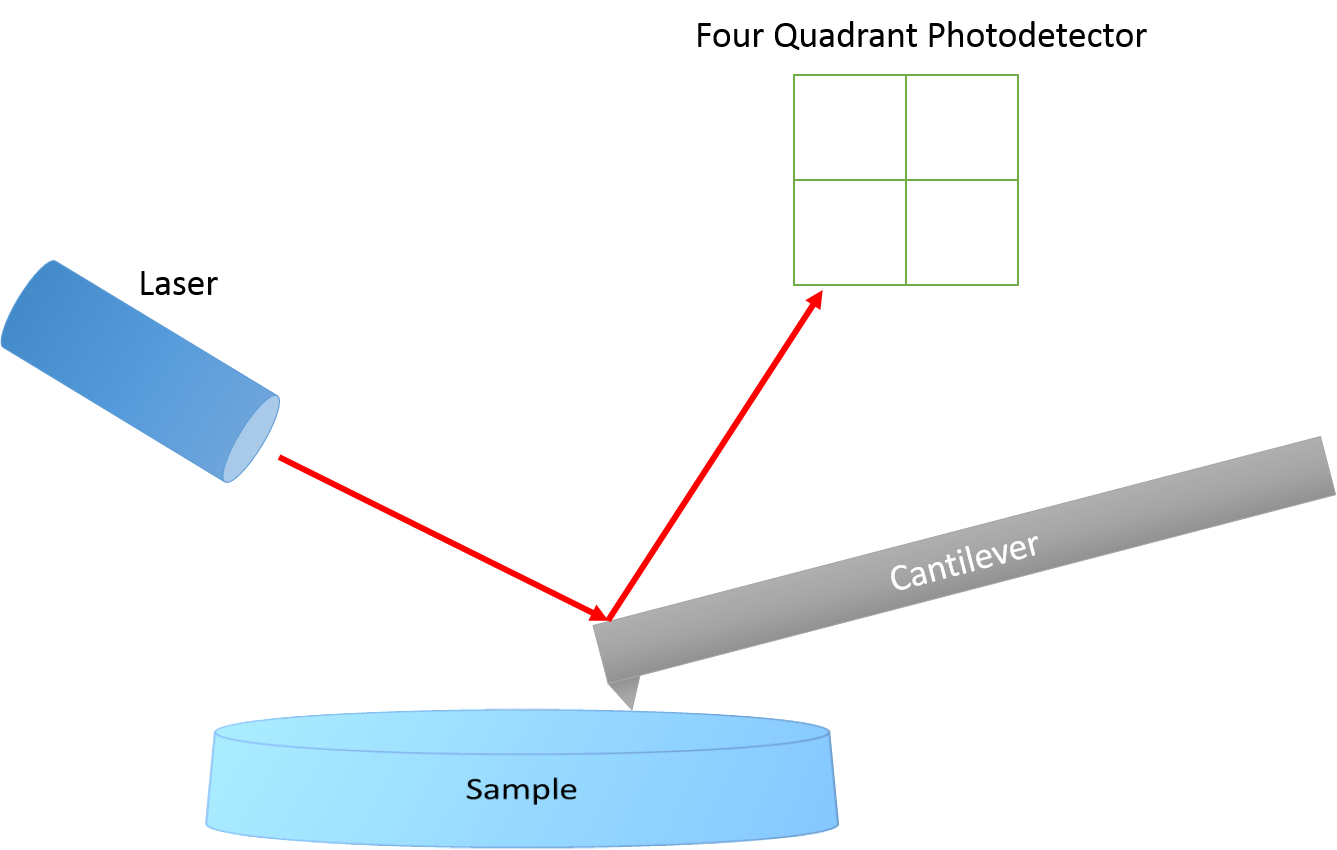
\includegraphics[width=0.7\textwidth]{Figs/Ch2/AFM.png}
	\caption {Schematic of an atomic force microscope.}
	\label{2.1}
\end{figure}
\FloatBarrier

The positioning and movement of the tip is achieved through the use of piezo-electric actuators. In contact mode, a feedback circuit is used to apply a voltage to the piezoelectric crystal in order to maintain a constant tip-sample separation should the tip encounter any features, thus avoiding damage to either the tip of sample. The voltage required to maintain this distance (also known as the setpoint) is registered at each pixel of the scan and is used in conjunction with calibration data to determine a vertical displacement value, thus generating a topographic image.\\
An alternative mode of operation known as tapping mode is often referred to contact mode. In this mode of operation the tip is made to oscillate close to its resonant frequency by the piezocrystal. Contact  between the tip and the sample is achieved at the lowest point of each oscillation, which damps the oscillation of the tip. The oscillation frequency is maintained by the piezoelectric crystal, thus allowing for the generation of a topographic map. Tapping mode is often preferred to contact mode due to the exclusion of lateral friction which can cause tip wear and sample damage.\\
The forces experienced by the tip vary depending on the tip-sample separation, as shown in Fig.\ref{2.2}. Van der Walls forces dominate at large separations attractive the tip to the surface. As the distance is reduced repulsive forces such as hard-sphere repulsion, electron-electron Coulomb interaction and the Pauli-exclusion interaction being to dominate. The sum of these forces result in cantilever deflection, changing the tip-sample interaction.

\begin{figure}[h]
	\centering
	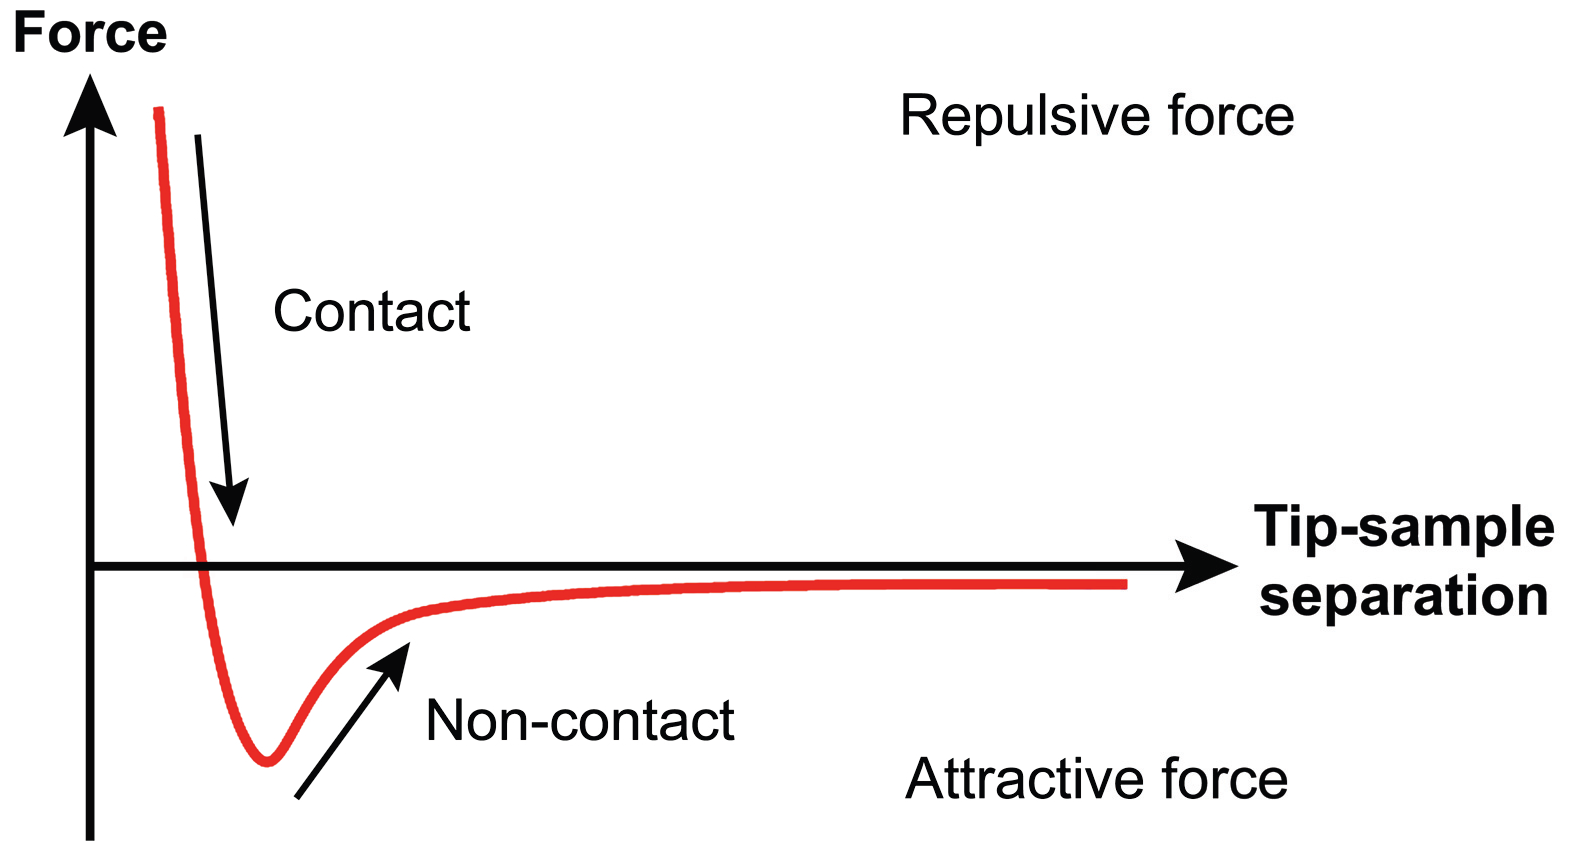
\includegraphics[width=0.7\textwidth]{Figs/Ch2/AFMint.png}
	\caption {The effect of separation on the tip-sample interaction force \cite{Zhu2010}.}
	\label{2.2}
\end{figure}
\FloatBarrier

AFM offers excellent vertical resolution limited only by the probes vertical movement and external noise. However, the lateral resolution of this microscopy technique is heavily dependent on the shape and size of the tip employed. This is perhaps best highlighted by Fig.\ref{2.3} which depicts a hemispherical tip scanning across a flat-topped island. The apex of the tip is in contact with the surface, but the side of the island also experiences some contact: in this case there is a distinction between the two cases shown in Fig.\ref{2.2}a) and b) as the error in the measured width of the island varies based on the relative size of the measured object to the tip.

\begin{figure}[h]
	\begin{subfigure}[t]{0.4\textwidth}
		\centering
		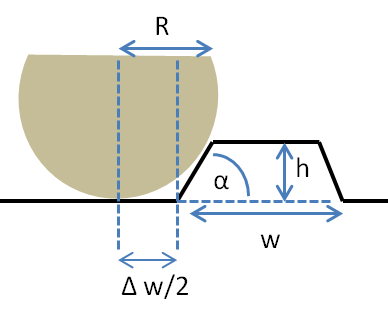
\includegraphics[width = 1\textwidth]{Figs/Ch2/afm1.png}
		\caption{}
	\end{subfigure}%
	\hspace*{1cm}
	~	
	\begin{subfigure}[t]{0.4\textwidth}
		\centering
		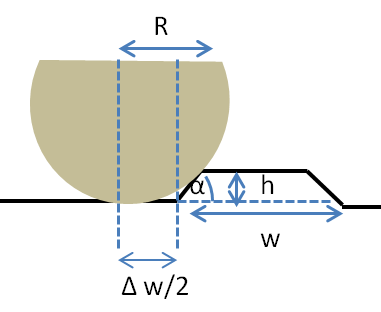
\includegraphics[width=1\textwidth]{Figs/Ch2/afm2.png}
		\caption{}
	\end{subfigure}
	\caption {Interaction of a hemisphere with a flat-topped island for the cases a) $h > R(1-cos(\alpha))$ and b) $h < R(1-cos(\alpha))$ adapted from \cite{Oliver2008}. }
	\label{2.3}
\end{figure}
\FloatBarrier 

Similarly, when measuring depth rather than height the ability of the tip to penetrate into the spaces being measured is also a crucial consideration, as shown in Fig.\ref{2.4}. Thus, increasing the gradient of the tip and minimizing the tip apex are descriable to reduce tip-related measurement artefacts when performing atomic force microscopy.

\begin{figure}[h]
	\centering
	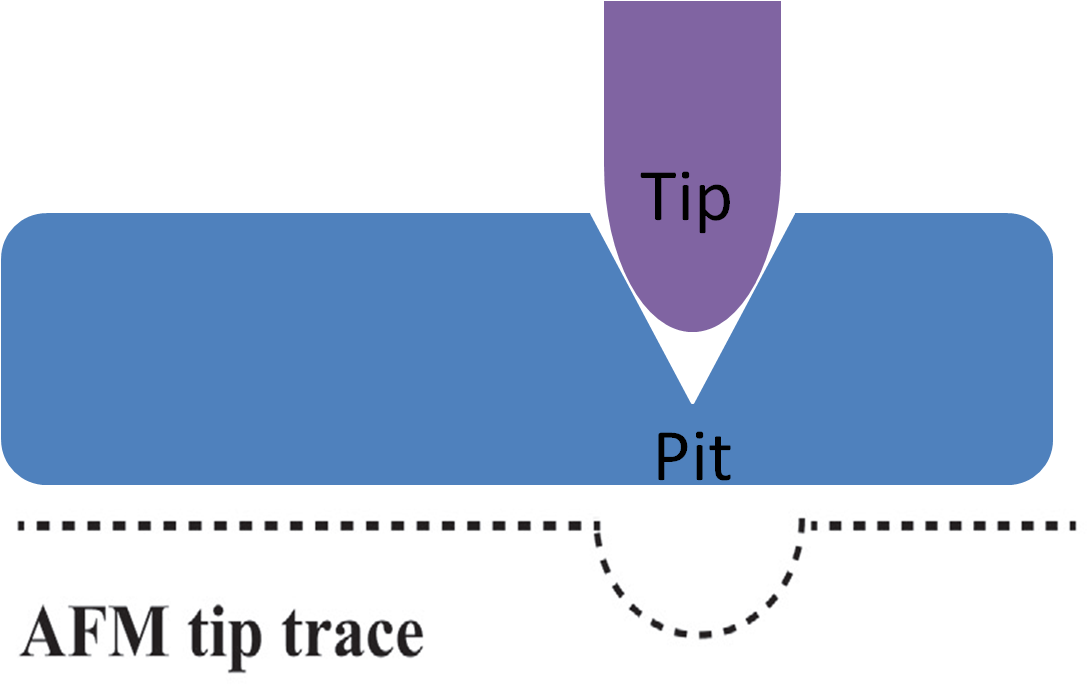
\includegraphics[width=0.4\textwidth]{Figs/Ch2/afm3.png}
	\caption {Measurement error in the depth of a pit caused by the finite width of the AFM tip.}
\end{figure}
\FloatBarrier

\subsubsection{Conductive Atomic Force Microcsopy}

Conductive atomic force microscopy \nomenclature[z-C-AFM]{C-AFM}{Conductive Atomic Force Microscopy} is a technique which combines AFM with local conductivity measurements. In order to perform C-AFM a conductive probe tip is brought close to contact with the sample and a bias is applied between the tip and the sample. The short tip-sample separation causes electron wavefunctions in the tip and sample to overlap, thus allowing a tunneling current to be generated through the application of a bias. C-AFM thus allows for the simultaneous measurement of tip-sample current flow and surface morphology, making it an extremely powerful tool to probe local sample conductivity. 


% Uncomment this line, when you have siunitx package loaded.
%The SI Units for dynamic viscosity is \si{\newton\second\per\metre\squared}.


\section{Scanning Electron Microscopy Techniques}

A scanning electron microscope  \nomenclature[z-SEM]{SEM}{Scanning Electron Microscope} (SEM) employs the use of electrons to characterise material morphology and composition. A schematic of a typical SEM design is shown in Fig.\ref{2.4}.

\begin{figure}[h]
	\centering
	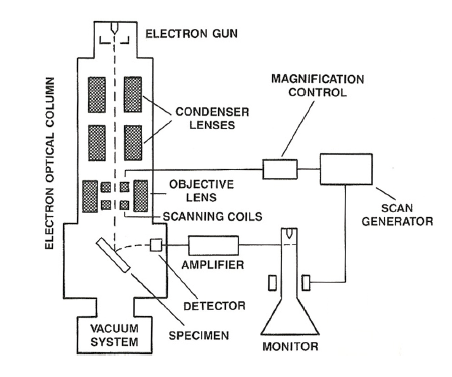
\includegraphics[width=0.6\textwidth]{Figs/Ch2/SEM.png}
	\caption {SEM design \cite{YacobiHolt1990}.}
	\label{2.4}
\end{figure}
\FloatBarrier

The electron gun generates a beam of electrons, typically of energy up to 30 keV. The condenser lenses situated below the gun serve to determine the probe size by adjusting the demagnification of the beam. The objective lens serves to further adjust this demagnification, and is situated directly above the specimen. The scanning coils serve to raster the electron probe across the sample, and the detector thus builds an image of the specimen by collecting various signals which occur due to the electron-specimen interactions.\\
As the beam of electrons interacts with the specimen, various processes occur which generate characteristic signals, as shown in Fig.\ref{2.5}. The volume within the sample which contains the energy deposited by the electron beam is known as the interaction volume, the shape and size of which is determined by both the beam energy and sample composition. Inelastic scattering of the electrons results in the production of signals such as secondary electrons \nomenclature[z-SE]{SE}{Secondary Electron} (SEs), Auger electrons and characteristic X-rays. Typically, it is the SEs which are used for imaging in SEMs. Elastic scattering can generate back scattered electrons \nomenclature[z-BSE]{BSE}{ Back Scattered Electron} (BSEs), which are collected through the surface on which the beam is incident. Due to the nature of elastic scattering, BSEs have a strong dependence on atomic, and are can thus be used to produce composition-dependent image contrast.

\begin{figure}[h]
	\centering
	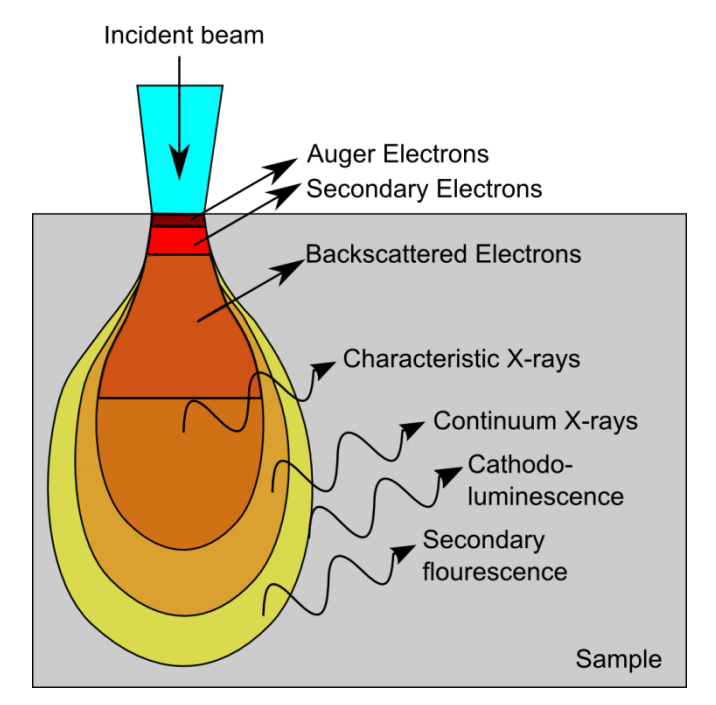
\includegraphics[width=0.6\textwidth]{Figs/Ch2/int.png}
	\caption {Interaction volumes for different interactions of an electron beam \cite{Puchtler2014}.}
	\label{2.5}
\end{figure}
\FloatBarrier



\subsubsection{Cathodoluminescence}

The absorption of primary electrons in a semiconductor can generate electronic excitations, or electron-hole pairs, with light emission occurring as a consequence of their recombination. This process is known as cathodoluminescence \nomenclature[z-CL]{CL}{Cathodoluminescence}(CL). The electronic transitions which are associated with CL emission require lower energies than those needed to excite X-rays.\\
\indent One of the principal advantages of CL in comparison with photo-excitation spectroscopy techniques used on semiconductors such as photoluminescence \nomenclature[z-PL]{PL}{Photoluminescence} (PL) is the limitation of the spatial resolution of the technique by the interaction volume of the elecctron beam in the material rather than diffraction which can be considered an intrinsic limitation of most optical far-field techniques \cite{Edwards2011}. As a result, nanometre-scale characterization of materials can be achieved.\\
\indent Due to the large number of electron-hole pairs generated within the interaction volume of the impinging electron beam on a bulk semiconductor material,all possible transitions within the material tend to be excited, resulting in the crucial limitation of being unable to selectively excite transitions below a certain energy \cite{Edwards2011}. Nonetheless, the versatility of CL as a technique has been amply demonstrated in its ability to shed light on the composition of compound materials such as InGaN/GaN structures \cite{Martin2004}, carrier diffusion length and surface recombination rates \cite{Sercel1989} and even minority carrier lifetimes \cite{YacobiHolt1990}.\\
\indent A schematic view of a set-up for CL imaging is show in Fig.\ref{2.6}:

\begin{figure}[!ht]
	\centering
	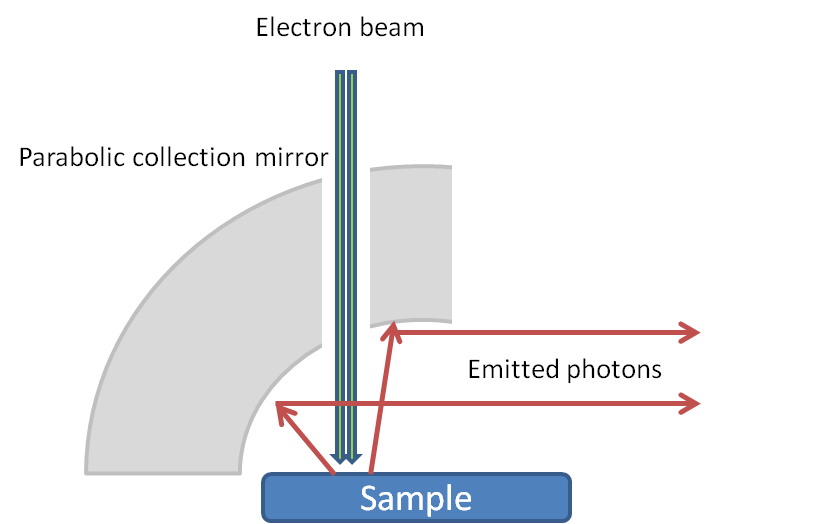
\includegraphics[width=0.5\textwidth]{Figs/Ch2/CL.png}
	\caption[h] {Schematic layout of a CL imaging system.}
	\label{2.6}
\end{figure}
\FloatBarrier

The electron beam is incident on the sample in the SEM chamber and results in the generation of photons which are collected by a parabolic mirror through a high vacuum feedthrough and coupled into a monochromator. Photomultiplier tubes (PMTs) are the most commonly used detector for this set-up. \\
The most basic form of CL imaging is known as panchromatic imaging. In this case, the collected light in its entirety is directed to a single detector and the resulting greyscale image intensity is the product of the spectral response of the system and the emission spectrum \cite{Edwards2011}. An extension of this is the monochromatic imaging mode, in which case only a single band of wavelengths is imaged using a band-pass filter or spectrometer \cite{Edwards2011}.\\
CL hyperspectral imaging, or CL wavelength imaging (CLWI) is an extension of the aforementioned technique whereby a full luminescence spectrum is recorded at each point during a beam scan, enabling the construction of a spatially and spectrally resolved data set.\\
 In the set-up shown in Fig \ref{2.6}, a semiparaboloidal mirror allows emitted photons to be collected over close to the entire hemisphere. In this case, the beam is scanned across the sample in order to achieve CL hyperspectral imaging, however a number of drawbacks are inherent to this collection geometry:\\
\\\indent - The position of the mirror requires a large working distance and can obscure the optical element thus compromising the imaging capabilities of the microscope.\\
\\\indent - The small distance between the sample and mirror imposes a restriction on the extent to which the sample can be tilted, which can be an issue in the examination of three-dimensional structures.\\
\\\indent - The {\it\'{e}tendue} of the system imposes a strict compromise between the field of view of the microscope and the collection efficiency at the spectrometer \cite{Edwards2011}.\\
\\\indent In an effort to overcome these limitations, CL hyperspectral imaging systems have been developed, whereby light collection is achieved using an objective placed perpendicular to the electron beam as shown below in Fig \ref{2.7}. By allowing the optics to be placed further away from the sample, a far shorter working distance can be used, allowing the electron spot to remain small at low accelerating voltages \cite{Edwards2011}. 

\begin{figure}[!ht]
	\centering
	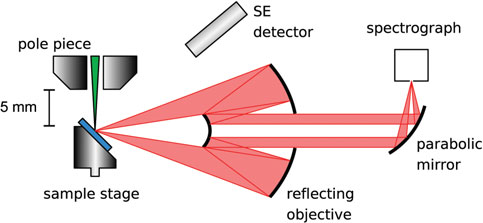
\includegraphics[width=0.5\textwidth]{Figs/Ch2/hyper.png}
	\caption[h] {Schematic layout of a CL hyperspectral imaging system \cite{Edwards2012}.}
	\label{2.7}
\end{figure}
\FloatBarrier

\subsubsection{Electron-Beam Induced Current}

Electron beam induced current \nomenclature[z-EBIC]{EBIC}{Electron-Beam Induced Current} (EBIC) imaging is a technique complementary to scanning electron microscopy. The premise of the measurement is that minority carriers which arise from the incident electron beam of an SEM on a semiconductor junction can diffuse to the junction where they are separated by the built-in field and collected as current by an external circuit (the EBIC amplifier).\\
Due to the small interaction volumes achievable, EBIC can provide detailed spatial information on minority carrier dynamics. Regions of high signal indicate high collection efficiency and low recombination, for example: the depletion region of a p-n junction appears bright in EBIC imaging. As such EBIC imaging has proven extremely useful in characterising the recombination properties of individual defects across a wide range of semiconductors \cite{Yakimov2002}.  


\section{Hyperspectral Electroluminescence Mapping}
\section{Photoluminescence}
\section{Dual Beam Scanning Electron microscopy with a Focussed Ion Beam}
\subsection{Fabrication}
\subsection{Tomography}
\section{Transmisson Electron Microscopy}
\subsection{Tomography}


